% Biên dịch bằng pdfLaTeX (mặc định của Overleaf).
\documentclass[12pt,a4paper]{article}
\usepackage[utf8]{inputenc}
\usepackage[T5]{fontenc}
\usepackage[vietnamese]{babel}
\usepackage{lmodern}
\usepackage[margin=2.5cm]{geometry}
\usepackage{booktabs,tabularx,array}
\usepackage{graphicx}
\usepackage{enumitem}
\usepackage{tikz}
\usetikzlibrary{positioning,arrows.meta,fit}
\usepackage[hidelinks]{hyperref}

\setlist{nosep,leftmargin=*}
\newcolumntype{L}{>{\raggedright\arraybackslash}X}
\newcommand{\spo}{SpO$_2$}
\newcommand{\code}[1]{\texttt{#1}}

\begin{document}

\begin{center}
  {\Large\bfseries BÁO CÁO TIẾN ĐỘ ĐỒ ÁN 2}\\[1ex]
  Giai đoạn: 01/09/2026 -- 01/11/2026 (đến tuần 45)
\end{center}

\noindent
\begin{tabularx}{\textwidth}{@{}lL@{}}
  \textbf{Đề tài:} & Xây dựng hệ thống giám sát tín hiệu sinh lý (EEG, nhịp tim, \spo) từ thiết bị đeo, sử dụng thiết bị biên và điện toán đám mây AWS, tích hợp trợ lý giọng nói \\
  \textbf{Sinh viên:} & \dots \quad \textbf{MSSV:} \dots \\
  \textbf{GVHD:} & \dots \\
\end{tabularx}

% ============================================================
\section{Mở đầu}

\subsection{Mục tiêu đề tài}

Xây dựng một hệ thống giám sát tín hiệu sinh lý, gồm bốn thành phần:
\begin{itemize}
  \item \textbf{Thiết bị đeo:} Muse 2 (EEG), Magene H303 (nhịp tim) và Yuwell YX110 (\spo).
  \item \textbf{Thiết bị biên Raspberry Pi 4:} thu nhận và xử lý tín hiệu ngay tại chỗ.
  \item \textbf{AWS:} lưu trữ và tổng hợp dữ liệu.
  \item \textbf{Web dashboard và trợ lý giọng nói:} người dùng xem chỉ số trên web, hoặc hỏi bằng giọng nói mà không cần dùng tay.
\end{itemize}

\subsection{Kết quả giai đoạn trước (hè 2026)}

\begin{itemize}
  \item Đã xây dựng web dashboard trên dữ liệu mẫu và bộ JSON Schema chuẩn hóa dữ liệu.
  \item Đã xây dựng pipeline trợ lý giọng nói (STT $\rightarrow$ LLM $\rightarrow$ TTS) chạy offline trên CPU. Sau khi benchmark, chọn cấu hình faster-distil-whisper-medium.en, qwen2.5:0.5b và Piper, giảm thời gian phản hồi từ khoảng 20\,s xuống dưới 5\,s mỗi lượt.
\end{itemize}

Bảng~\ref{tab:ke-hoach} đối chiếu kế hoạch đặt ra cuối kỳ hè với tình hình thực hiện.

\begin{table}[h]
  \centering
  \caption{Kế hoạch cuối kỳ hè và tình hình thực hiện}
  \label{tab:ke-hoach}
  \begin{tabularx}{\textwidth}{@{}lL@{}}
    \toprule
    Kế hoạch cuối kỳ hè & Tình hình trong giai đoạn này \\
    \midrule
    Triển khai AWS Services & \textbf{Đang thực hiện} (mục~\ref{sec:aws}) \\
    Kết nối Mobile App và Google Health Connect & \textbf{Thay đổi hướng.} Bỏ đồng hồ Galaxy Fit 3 và Health Connect; mọi thiết bị đeo kết nối thẳng vào Raspberry Pi (mục~\ref{sec:kien-truc}) \\
    Đo lại pipeline giọng nói trên Raspberry Pi 4 & \textbf{Chưa thực hiện}, vì giai đoạn này ưu tiên đường dữ liệu từ thiết bị đeo \\
    \bottomrule
  \end{tabularx}
\end{table}

\subsection{Phạm vi công việc trong kỳ báo cáo}

Giai đoạn này tập trung vào \textbf{đường dữ liệu từ thiết bị đeo lên cloud}, làm theo hướng ``lát cắt dọc nhỏ nhất'': cho dữ liệu thật đi được từ cảm biến tới web trước, rồi mới hoàn thiện từng phần. Gồm các việc:
\begin{enumerate}
  \item thiết kế lại kiến trúc;
  \item thu nhận dữ liệu từ ba thiết bị đeo;
  \item chương trình xử lý trên thiết bị biên;
  \item backend AWS (đang làm);
  \item nối web dashboard với dữ liệu thật.
\end{enumerate}

% ============================================================
\section{Tóm tắt tiến độ theo mốc thời gian}

\begin{table}[h]
  \centering
  \caption{Tiến độ theo mốc thời gian}
  \begin{tabularx}{\textwidth}{@{}p{2.4cm}p{3cm}L@{}}
    \toprule
    Thời gian & Hạng mục & Nội dung chính \\
    \midrule
    01/09 -- 19/09 & \dots & \textit{(TODO: điền việc đã làm; giai đoạn này git không có commit)} \\
    20/09 -- 28/09 & Thiết kế, schema & Chốt kiến trúc mới, trong đó Raspberry Pi là cổng dữ liệu duy nhất; cập nhật schema. Dựng thử backend AWS rồi gỡ bỏ để làm lại theo kiến trúc mới. Chuyển máy phát triển sang Ubuntu 26.04 \\
    26/10 & Thu nhận dữ liệu & Chương trình đọc BLE kèm dashboard riêng cho từng thiết bị \\
    27/10 -- 28/10 & Thiết bị biên, AWS & Chạy đồng thời 3 thiết bị trên Pi. Đo phiên mắt mở/mắt nhắm. Viết \code{gateway.py}. Dựng API \code{/sessions}. Pi gửi phiên đo đầu tiên lên AWS \\
    29/10 & AWS, web & Gửi dữ liệu tự động mỗi phút, giả lập mất mạng, web đọc dữ liệu từ API. Thêm \code{/measurements}, tổng hợp hằng đêm và \code{/vitals/latest} \\
    30/10 -- 01/11 & Web & Chuyển web sang đọc tổng hợp theo ngày từ \code{/vitals/daily} (đang làm) \\
    \bottomrule
  \end{tabularx}
\end{table}

Số liệu từ git: 24 commit, khoảng 11.900 dòng thêm và 1.500 dòng xóa.

% ============================================================
\section{Thiết kế hệ thống và thu nhận dữ liệu}

\subsection{Thay đổi kiến trúc}
\label{sec:kien-truc}

\begin{itemize}
  \item \textbf{Lý do thay đổi.} Bỏ đồng hồ Galaxy Fit 3 và Google Health Connect, vì \dots\ \textit{(TODO: điền lý do)}.
  \item \textbf{Thiết bị thay thế:}
  \begin{itemize}
    \item \textbf{Magene H303}, đai ngực đo ECG, cho nhịp tim và RR interval;
    \item \textbf{Yuwell YX110}, kẹp ngón tay, đo \spo.
  \end{itemize}
  \item \textbf{Kiến trúc mới:} cả ba thiết bị kết nối BLE thẳng vào Raspberry Pi 4. Pi là \textbf{cổng dữ liệu duy nhất} lên AWS (Hình~\ref{fig:kien-truc}).
  \item \textbf{Quy tắc chọn nguồn khi nhiều thiết bị cùng đo một chỉ số:}
  \begin{itemize}
    \item nhịp tim lấy H303 trước, sau đó PPG của Muse 2, cuối cùng YX110;
    \item \spo{} chỉ lấy từ YX110.
  \end{itemize}
\end{itemize}

\begin{figure}[h]
  \centering
  \begin{tikzpicture}[
      font=\small,
      box/.style={draw, rounded corners, align=center, minimum height=1cm, inner sep=4pt},
      dev/.style={box, minimum width=2.2cm},
      arr/.style={-{Stealth}, thick},
      node distance=0.4cm and 0.9cm]
    \node[dev] (muse) {Muse 2\\EEG, PPG};
    \node[dev, below=of muse] (h303) {Magene H303\\nhịp tim, RR};
    \node[dev, below=of h303] (yx) {Yuwell YX110\\\spo};
    \node[box, right=of h303, text width=3.6cm] (pi) {\textbf{Raspberry Pi 4}\\(thiết bị biên)\\[2pt]
      \footnotesize giải mã, 72 đặc trưng EEG, tóm tắt phiên, hàng đợi SQLite, gửi lên mỗi phút};
    \node[box, right=of pi, text width=2.8cm] (aws) {\textbf{AWS}\\[2pt]
      \footnotesize API Gateway, Lambda, DynamoDB};
    \node[box, right=of aws, yshift=0.9cm, minimum width=2.4cm] (web) {Web\\dashboard};
    \node[box, right=of aws, yshift=-0.9cm, minimum width=2.4cm, dashed] (voice) {Trợ lý\\giọng nói};
    \foreach \d in {muse,h303,yx} \draw[arr] (\d.east) -- (pi.west);
    \node[above=0.1cm of pi.north west, anchor=south east, font=\footnotesize] {BLE};
    \draw[arr] (pi) -- node[above, font=\footnotesize] {HTTPS} (aws);
    \draw[arr] (aws) -- (web);
    \draw[arr, dashed] (aws) -- (voice);
  \end{tikzpicture}
  \caption{Kiến trúc hệ thống. Nét đứt: phần chưa kết nối.}
  \label{fig:kien-truc}
\end{figure}

\subsection{Cập nhật schema dữ liệu}

\begin{itemize}
  \item Thêm \code{spot\_measurement\_schema.json} cho số đo \spo.
  \item Sửa \code{daily\_vitals\_schema.json}: AWS tính bản ghi này mỗi đêm; bỏ số bước chân; thêm trường thiết bị nguồn.
  \item Mở rộng \code{active\_session\_schema.json}: thêm danh sách thiết bị và RR interval của H303.
  \item Bổ sung test kiểm tra schema vào \code{validate\_schemas.py}.
\end{itemize}

\subsection{Thu nhận dữ liệu từ ba thiết bị đeo}

\begin{table}[h]
  \centering
  \caption{Giao thức và kết quả thu nhận của từng thiết bị}
  \begin{tabularx}{\textwidth}{@{}p{2.6cm}p{4.4cm}L@{}}
    \toprule
    Thiết bị & Giao thức & Kết quả \\
    \midrule
    Magene H303 & Heart Rate Service chuẩn (\code{0x180D}) & Đọc nhịp tim và RR interval, không cần ghép đôi (pair) \\
    Yuwell YX110 & Giao thức riêng (\code{ffe0}/\code{ffe4}), không theo chuẩn Pulse Oximeter & Tự giải mã gói 10 byte gồm \spo, nhịp mạch và checksum \\
    Muse 2 & GATT riêng (\code{0xFE8D}) & Thu đủ các luồng: EEG 4 kênh 256\,Hz, PPG 3 kênh 64\,Hz, accelerometer, gyroscope, pin \\
    \bottomrule
  \end{tabularx}
\end{table}

Muse 2 đo thật trong 140 giây: tốc độ mẫu khớp thông số của thiết bị và \textbf{không mất gói nào}.

% Gợi ý hình: ảnh chụp thật ba thiết bị đeo và Raspberry Pi.
% \begin{figure}[h]
%   \centering
%   \includegraphics[width=0.7\textwidth]{figures/thiet-bi.jpg}
%   \caption{Ba thiết bị đeo và Raspberry Pi 4}
% \end{figure}

\subsection{Chạy đồng thời ba thiết bị trên Raspberry Pi}

Đo 10 phút, cả ba thiết bị chạy trên cùng một adapter Bluetooth (Bảng~\ref{tab:dong-thoi}).

\begin{table}[h]
  \centering
  \caption{Chạy đồng thời ba thiết bị trong 10 phút}
  \label{tab:dong-thoi}
  \begin{tabularx}{\textwidth}{@{}Lcc@{}}
    \toprule
    Chỉ số & PC Ubuntu (đối chứng) & Raspberry Pi 4, Wi-Fi bật \\
    \midrule
    Muse 2: số lần rớt kết nối & 1 & \textbf{0} \\
    Muse 2: khoảng không nhận được gói dài nhất & 9,4\,s & \textbf{0,2\,s} \\
    H303: số lần rớt kết nối & 0 & 0 \\
    Ping tới Pi trong lúc đo & -- & không mất gói \\
    \bottomrule
  \end{tabularx}
\end{table}

\textbf{Kết luận:} Wi-Fi và Bluetooth của Pi 4 dùng chung một chip nhưng chạy cùng lúc vẫn ổn, nên không cần mua USB Bluetooth.

\subsection{Kiểm tra chất lượng tín hiệu}

\textbf{Quy trình đo:} nghỉ 1 phút, rồi mở mắt và nhắm mắt luân phiên, mỗi đoạn 2 phút, lặp 2 lần.

\begin{table}[h]
  \centering
  \caption{Tỉ lệ công suất sóng alpha (8--12\,Hz) khi nhắm mắt so với khi mở mắt}
  \label{tab:alpha}
  \begin{tabular}{@{}cccc@{}}
    \toprule
    TP9 & AF7 & AF8 & TP10 \\
    \midrule
    \textbf{3,17} & 0,79 & 0,90 & \textbf{2,47} \\
    \bottomrule
  \end{tabular}
\end{table}

Alpha chỉ tăng ở hai kênh sau tai (TP9, TP10), đúng phân bố sinh lý của sóng alpha ở vùng sau đầu (Bảng~\ref{tab:alpha}). Khi nhắm mắt, phổ của TP9 và TP10 có đỉnh rõ quanh 11\,Hz, còn AF7 và AF8 không có (Hình~\ref{fig:alpha}). Như vậy Muse 2 ghi EEG đúng.

\begin{figure}[h]
  \centering
  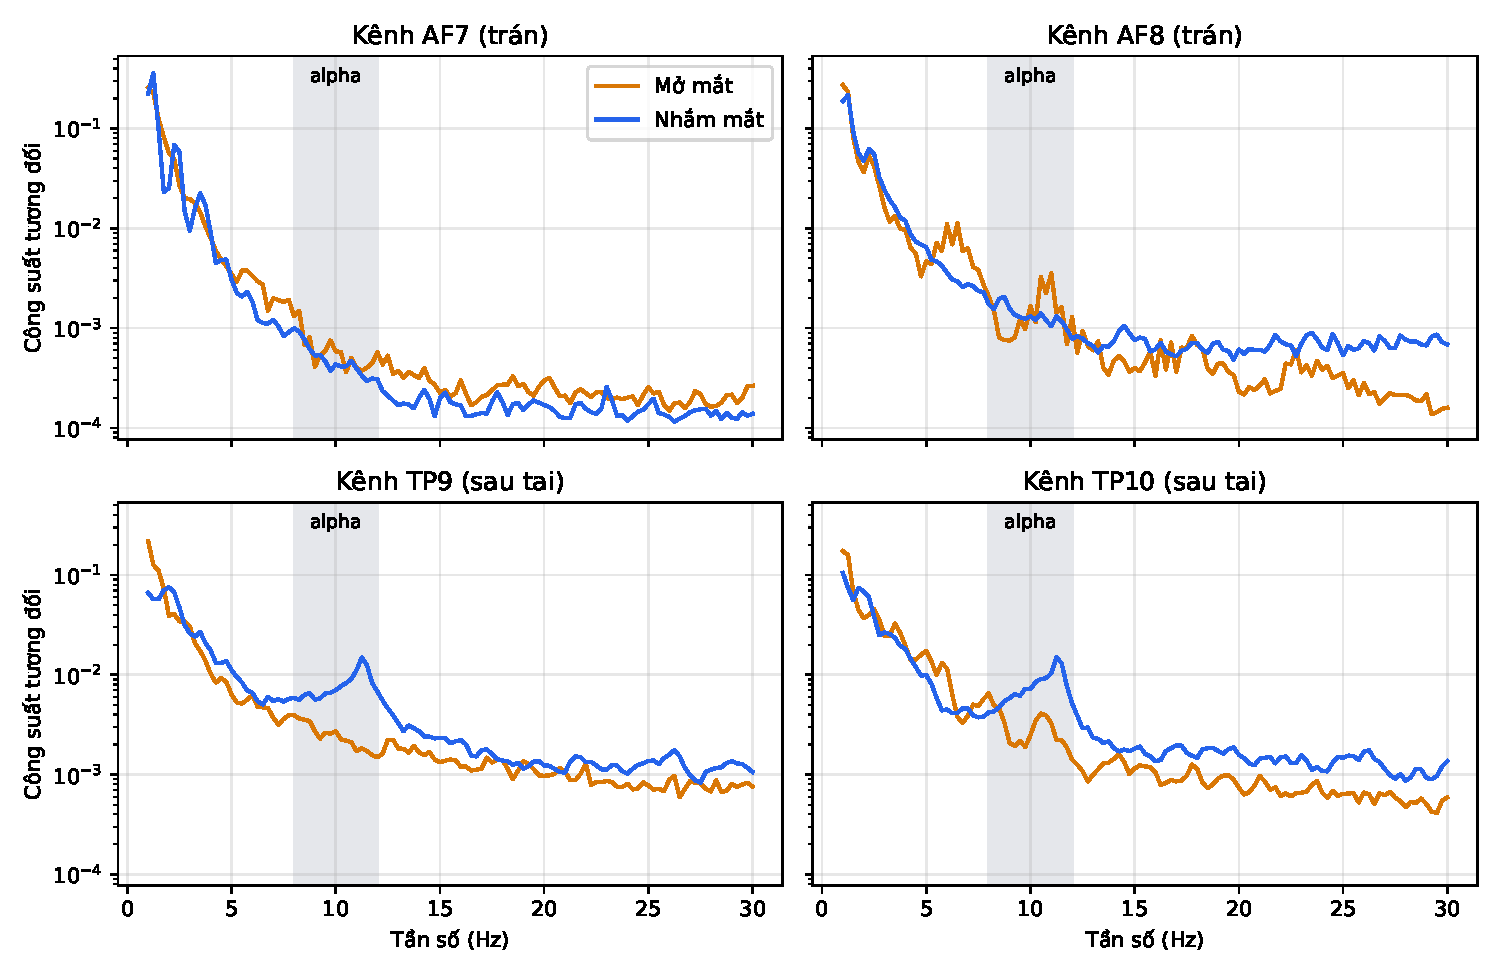
\includegraphics[width=\textwidth]{figures/alpha-psd.pdf}
  \caption{Phổ công suất tương đối (chia cho tổng công suất 1--40\,Hz) của 4 kênh EEG Muse 2, trung bình hai lần mở mắt và hai lần nhắm mắt. Vùng tô xám: dải alpha 8--12\,Hz.}
  \label{fig:alpha}
\end{figure}

\begin{table}[h]
  \centering
  \caption{Nhịp tim theo từng giai đoạn (BPM)}
  \begin{tabular}{@{}lccc@{}}
    \toprule
    Giai đoạn & Muse 2 PPG & H303 & YX110 \\
    \midrule
    Mở mắt 1 & 54,9 & 71,8 & 71,9 \\
    Nhắm mắt 1 & 71,1 & 71,9 & 71,6 \\
    Mở mắt 2 & 68,6 & 69,3 & 69,6 \\
    Nhắm mắt 2 & 72,5 & 72,8 & 73,0 \\
    \bottomrule
  \end{tabular}
\end{table}

\begin{itemize}
  \item H303 và YX110 lệch nhau dưới 0,3\,BPM.
  \item PPG của Muse 2 kém tin cậy hơn, có đoạn lệch tới hơn 20\,BPM (Hình~\ref{fig:nhip-tim}), nên chỉ dùng làm tham khảo; \textbf{nguồn nhịp tim chính là H303}.
\end{itemize}

\begin{figure}[h]
  \centering
  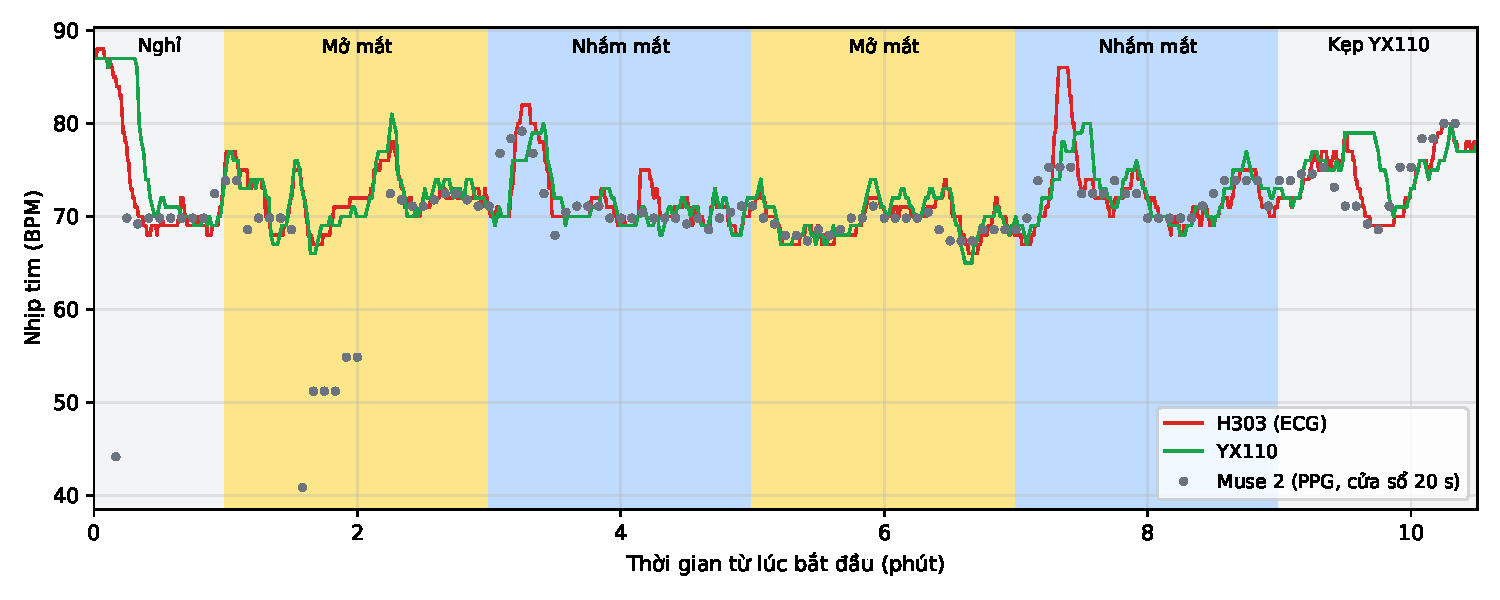
\includegraphics[width=\textwidth]{figures/nhip-tim.pdf}
  \caption{Nhịp tim theo thời gian của ba thiết bị trong phiên đo ngày 28/10/2026. Muse 2: mỗi điểm ước tính từ một cửa sổ PPG 20\,s.}
  \label{fig:nhip-tim}
\end{figure}

% ============================================================
\section{Chương trình trên thiết bị biên và backend AWS}

\subsection{Chương trình xử lý trên thiết bị biên (\code{gateway.py})}

Một tiến trình duy nhất chạy trên Raspberry Pi:
\begin{itemize}
  \item kết nối cả ba thiết bị và tự kết nối lại khi rớt;
  \item mỗi giây ghi vào hàng đợi SQLite:
  \begin{itemize}
    \item \textbf{72 đặc trưng EEG}: 4 kênh $\times$ 18 đặc trưng (công suất các dải tần, tỉ lệ $\theta/\alpha/\beta$, chỉ số Hjorth, SEF95, spectral entropy), tính trên cửa sổ 4 giây sau lọc notch 50\,Hz;
    \item nhịp tim;
    \item \spo;
  \end{itemize}
  \item khi kết thúc mỗi phiên, tạo bản tóm tắt theo schema \code{active\_session};
  \item ghi dữ liệu thô vào thẻ SD (khoảng 75\,MB/giờ).
\end{itemize}

Có test cho phần tính đặc trưng và tóm tắt phiên. Kết quả chạy thử 10 phút trên Pi ở Bảng~\ref{tab:gateway}.

\begin{table}[h]
  \centering
  \caption{Chạy thử \code{gateway.py} 10 phút trên Raspberry Pi}
  \label{tab:gateway}
  \begin{tabularx}{\textwidth}{@{}lL@{}}
    \toprule
    Hạng mục & Kết quả \\
    \midrule
    Kết nối & Cả ba thiết bị, không rớt lần nào \\
    Đặc trưng EEG & 546 dòng, đủ 72 đặc trưng, không có giá trị lỗi \\
    Nhịp tim từ H303 & 518 dòng, 70,7--81,7\,BPM \\
    Nhịp tim từ PPG của Muse 2 & Lệch trung vị 1,7\,BPM so với H303 \\
    \spo{} từ YX110 & 594 dòng, 96--100\,\% \\
    \bottomrule
  \end{tabularx}
\end{table}

\subsection{Gửi dữ liệu từ Pi lên AWS}

\begin{itemize}
  \item \code{upload.py} chạy bằng cron mỗi phút. Nó gửi các phiên và số đo chưa gửi, rồi đánh dấu trạng thái: đã gửi, chưa gửi, hoặc bị server từ chối.
  \item \textbf{Giả lập mất mạng} bằng cách gửi tới một địa chỉ không tồn tại: dữ liệu vẫn nằm trong hàng đợi. Khi có mạng lại, nó được gửi bù \textbf{đúng một lần}.
  \item Đã gửi lên AWS 2 phiên đo thật và 231 số đo \spo, không số đo nào bị từ chối.
\end{itemize}

\subsection{Backend AWS (đang thực hiện)}
\label{sec:aws}

Dựng bằng AWS SAM: API Gateway (bắt buộc API key), Lambda Python và DynamoDB.

\begin{table}[h]
  \centering
  \caption{Trạng thái các thành phần backend AWS}
  \begin{tabularx}{\textwidth}{@{}Lp{4.6cm}@{}}
    \toprule
    Thành phần & Trạng thái \\
    \midrule
    \code{POST/GET /sessions}: lưu và đọc tóm tắt phiên đo, có kiểm tra schema và không tạo bản ghi trùng & Đã chạy với dữ liệu thật \\
    \code{POST/GET /measurements}: nhận số đo \spo{} theo lô; số đo sai bị từ chối riêng lẻ & Đã chạy với dữ liệu thật \\
    Tổng hợp chỉ số mỗi đêm và \code{GET /vitals/daily} & Đã viết và có test, chưa kiểm tra trọn vẹn \\
    \code{GET /vitals/latest}: chỉ số mới nhất cho trợ lý giọng nói & Đã viết và có test, chưa nối với trợ lý \\
    Lưu dữ liệu thô lên S3 & Chưa làm \\
    Đăng nhập người dùng (Cognito) & Chưa làm. Hiện dùng một người dùng cố định và API key \\
    Cảnh báo bất thường & Chưa làm \\
    CI/CD tự động deploy & Chưa làm \\
    \bottomrule
  \end{tabularx}
\end{table}

\subsection{Web dashboard}

\begin{itemize}
  \item Đọc phiên mới nhất từ API thay cho file mẫu. Đã kiểm tra trên Chrome: hiện nhịp tim 73,7\,BPM lấy từ API, mở cả 4 tab không có lỗi.
  \item Đang chuyển thẻ chỉ số theo ngày sang đọc từ \code{/vitals/daily}.
  \item Các thẻ hồ sơ, huyết áp, hoạt động và cảnh báo vẫn đọc dữ liệu mẫu, vì chưa có API hay thiết bị đo tương ứng.
\end{itemize}

% Gợi ý hình: ảnh chụp web dashboard đang hiện phiên đo thật lấy từ API.
% \begin{figure}[h]
%   \centering
%   \includegraphics[width=\textwidth]{figures/web-dashboard.png}
%   \caption{Web dashboard hiện phiên đo thật lấy từ API}
% \end{figure}

% ============================================================
\section{Khó khăn và giải pháp kỹ thuật}

\begin{table}[h]
  \centering
  \caption{Khó khăn và giải pháp}
  \begin{tabularx}{\textwidth}{@{}p{5.6cm}L@{}}
    \toprule
    Khó khăn & Giải pháp \\
    \midrule
    YX110 không theo chuẩn Pulse Oximeter Service của Bluetooth & Phân tích cách ứng dụng chính hãng xử lý dữ liệu để giải mã gói 10 byte. Kiểm tra checksum để loại gói lỗi \\
    Lo ngại Wi-Fi và Bluetooth dùng chung chip trên Pi 4 sẽ làm rớt kết nối & Viết công cụ đo đồng thời 10 phút để có số liệu trước khi quyết định. Kết quả: không cần mua USB Bluetooth \\
    PPG của Muse 2 cho nhịp tim sai lệch & Chọn H303 làm nguồn chính và lọc các nhịp không đều. Tỉ lệ số giây PPG lệch không quá 5\,BPM so với H303 tăng từ 87\,\% lên 97\,\% \\
    Pi có thể mất mạng khi đang đo & Dùng hàng đợi SQLite trên Pi; mỗi bản ghi có khóa duy nhất nên gửi lại không tạo bản ghi trùng \\
    Backend AWS dựng lần đầu (20/09) quá rộng và không khớp kiến trúc mới & Gỡ bỏ và làm lại theo hướng lát cắt dọc: chỉ thêm API khi có dữ liệu thật cần dùng \\
    Dữ liệu lưu theo giờ UTC, còn người dùng ở UTC+7 & Tính ``một ngày'' theo giờ Việt Nam khi tổng hợp chỉ số hằng đêm \\
    \bottomrule
  \end{tabularx}
\end{table}

% ============================================================
\section{Hạn chế hiện tại}

\begin{itemize}
  \item \textbf{Backend AWS chưa hoàn thành:} còn thiếu S3, Cognito, cảnh báo và CI/CD; phần tổng hợp hằng đêm chưa được kiểm tra trọn vẹn.
  \item Chưa kiểm tra trọn đường với thiết bị thật sau khi bật gửi tự động, tức là đeo thiết bị rồi thấy phiên tự hiện trên web.
  \item Kiểm tra mất mạng mới là giả lập, chưa ngắt Wi-Fi thật.
  \item \textbf{Trợ lý giọng nói chưa nối với dữ liệu thật}, và chưa được đo lại trên Raspberry Pi 4.
  \item Chưa có phân giai đoạn giấc ngủ từ EEG; điểm tổng hợp của phiên (\code{overall\_score}) chưa được định nghĩa.
  \item Không có thiết bị đo huyết áp.
  \item Cách chia 72 đặc trưng EEG do em tự đặt, cần thầy/cô góp ý.
\end{itemize}

% ============================================================
\section{Kế hoạch tiếp theo}

\begin{enumerate}
  \item Hoàn thành backend AWS: kiểm tra trọn vẹn phần tổng hợp hằng đêm, sau đó làm S3 cho dữ liệu thô.
  \item Hoàn thành web đọc chỉ số theo ngày từ \code{/vitals/daily}.
  \item Nối trợ lý giọng nói với \code{/vitals/latest}, để người dùng hỏi được nhịp tim và \spo{} gần nhất bằng giọng nói.
  \item Kiểm tra trọn đường với thiết bị thật, kể cả ngắt Wi-Fi thật.
  \item Định nghĩa \code{overall\_score} và quyết định phạm vi phân giai đoạn giấc ngủ.
  \item Nếu còn thời gian: Cognito, cảnh báo, ứng dụng di động dạng PWA.
\end{enumerate}

\end{document}
